\section{Ethical Considerations}

The deep learning model aimed to be implemented during this project will require real-life data to learn its underlying patterns in order to be able to detect cases of breast cancer in mammograms and to evaluate its performance. Therefore, the main ethical concern when using sensitive medical data such as  mammograms is whether it can be traced back to the original patient. As a result, fully anonymous, open-source and public datasets are used. A full Ethics Application to the University of St Andrew's Teaching and Research Ethics Committee was therefore submitted at the early stages of the project and later approved. The approval letter from the committee can be found in Appendix~\ref{ch:appendix-ethical-approval-letter}.

%%%%%%%%%%%%%%%%%%%%%%%%%%%%%%%%%%%%%%%%%%%%%%%%%%%%%%

\section{Datasets Description}

Three open-sourced anonymised public datasets have been approved by the University of St Andrew's Teaching and Research Ethics Committee for use in this project.

\subsection{DDSM}

The ``Digital Database for Screening Mammography'' (DDSM) dataset is a dataset initially released in 2007 and available online from the University of Florida. It holds 2,620 scanned film mammography of normal, benign and malignant cases, all stored in Lossless JPEG format (LJPEG), which is obsolete nowadays \citep{MichaelHeathKevinBowyerDanielKopans2001}.

\subsection{CBIS-DDSM}
\label{sec:ethics-datasets-cbisddsm}

The ``Curated Breast Imaging Subset of DDSM'' (CBIS-DDSM) dataset \citep{Lee2017} is available online from The Cancer Imaging Archive \citep{Clark2013}. The dataset contains a total of 10,239 images in Digital Imaging and Communications in Medicine format (DICOM) gathered from 1,566 patients across 6,775 studies \citep{Lee2017}. This dataset is an updated and standardised subset of the older DDSM dataset \citep{DDSMdataset2001}, containing only abnormal cases with benign and malignant tumours (no normal cases).

\begin{figure}[ht]
\centerline{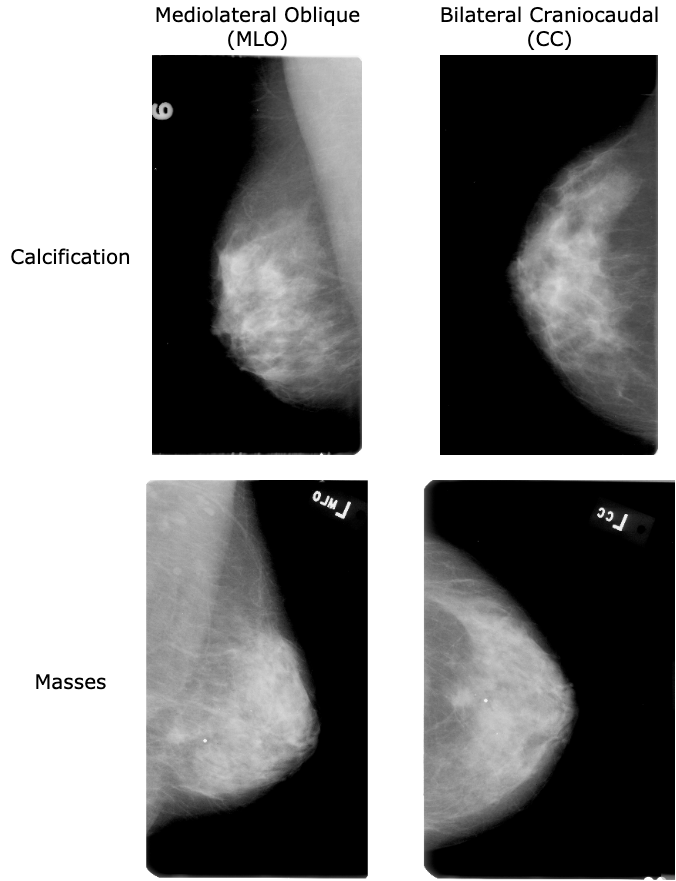
\includegraphics[width=0.8\textwidth]{figures/ethics-datasets/CBIS-DDSM views_types.png}}
\caption{\label{fig:ethics-datasets-CBIS-DDSM views_types}Types of structures and views captured by the CBIS-DDSM dataset (CC and MLO mammogram views are from the same patient).}
\end{figure}

The scans are a mix of the two most commonly used projections in routine mammogram X-ray scans: bilateral craniocaudal (CC) and mediolateral oblique (MLO) \citep{Elter2009}. The dataset can be further be separated into two different types of structures that radiologists usually look for to detect early signs of breast cancer: calcifications (small flecks of calcium usually clustered together) and masses (e.g. cysts or lumps) \citep{breastcancerorg2018}. Figure~\ref{fig:ethics-datasets-CBIS-DDSM views_types} illustrates the different type of mammograms found in the dataset.
% https://radiopaedia.org/articles/mammography-views

\subsection{mini-MIAS}
\label{sec:ethics-mini-MIAS-dataset-description}

The ``mini Mammography Image Analysis Society'' dataset (mini-MIAS) is a smaller dataset of mammograms containing 322 images in greyscale Portable Gray Map (PGM) format with associated ground truth data \citep{Suckling1994} and images all reduced to uniform size of 1024 x 1024 pixels \citep{Vishrutha2014}. The dataset contains three different types of mammograms: glandular dense, fatty and fatty glandular (see Figure~\ref{fig:ethics-datasets-mini-mias breast background}), which are further divided into normal, benign and malignant cases \citep{Hepsag2017}.

\begin{figure}[ht]
\centerline{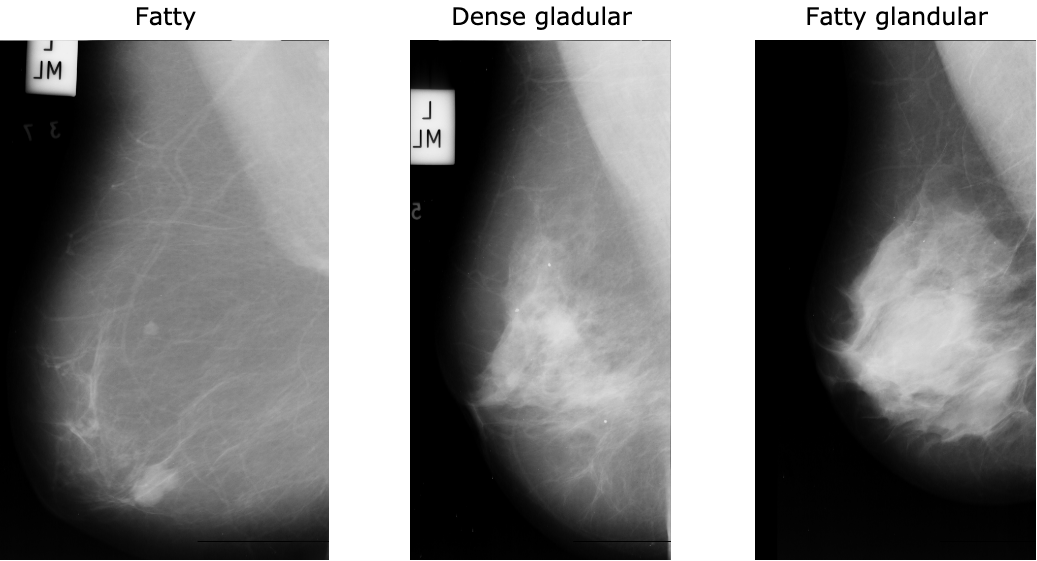
\includegraphics[width=\textwidth]{figures/ethics-datasets/mini-mias breast background.png}}
\caption{\label{fig:ethics-datasets-mini-mias breast background}The three different types of breast background found in the mini-MIAS dataset.}
\end{figure}